\def\year{2019}\relax
%File: formatting-instruction.tex
\documentclass[letterpaper]{article} %DO NOT CHANGE THIS
\usepackage{aaai19} %Required
\usepackage{times} %Required
\usepackage{helvet} %Required
\usepackage{courier} %Required
\usepackage{url} %Required
\usepackage{graphicx} %Required
\usepackage{amssymb}
\usepackage{amsmath}
\usepackage{mathrsfs}
\usepackage{multirow}
\usepackage{CJKutf8}
\usepackage{color}
\usepackage[table,xcdraw]{xcolor}
% \usepackage{xcolor}%定义了一些颜色
\usepackage{colortbl,booktabs}%第二个包定义了几个*rule
% \usepackage{multirow}
% https://www.tablesgenerator.com/
\graphicspath{{./picture/}}
\frenchspacing %Required
\setlength{\pdfpagewidth}{8.5in} %Required
\setlength{\pdfpageheight}{11in} %Required
\newcommand{\KZ}[1]{{\bf \color{red} KZ: #1}}

% \graphicspath{{./fig/}}
%PDF Info Is Required:
 \pdfinfo{
/Title (2019 Formatting Instructions for Authors Using LaTeX)
/Author (AAAI Press Staff)}
\setcounter{secnumdepth}{0} 
 \begin{document}
% The file aaai.sty is the style file for AAAI Press 
% proceedings, working notes, and technical reports.

% \title{Collaboration Gate Attention for E-commerce Recommendation Text Generation}
\title{GMA: Gated Memory Attention for E-Commerce Item Description Generation}
\author{AAAI Press
}
\maketitle
\begin{abstract}

% 消融学习。
% gma的核心创新点

% 解决什么问题
% 解决问题提出的方法
% 解决问题得到了什么结果
% 结果有什么理论或实际影响
\KZ{If the paper is about solving repetition problem in the generated
description, this should be said explicitly in the title of the paper.
So consider changing the title to be more expressive. Also the abstract is
too verbose right now. Just 4 sentences will do. Don't include how you solve
the problem. Just state what the problem is and your major contributions.}
With the advancement and popularity of E-Commerce, item description becomes increasingly important in the business scenario, 
for its role in information transferring and customer-attracting.
In this paper, we introduce a new problem, namely E-Commerce item description generation (EC-IDG), to the research community of neural language generation (NLG).
Repetition problem is often encountered in NLG problems, especially for EC-IDG, in which long sentence descriptions are generated from short attributes (key) words.
We propose a novel network, named gated memory attention (GMA), to solve the repetition problem of EC-IDG.
The proposed GMA network mainly consists of source attention, memory attention, and gated selection. 
Memory attention module contains two memory blocks that store hidden state of previous prediction.
During description generation, GMA first applies source attention and memory attention to generate context vector and memory vectors, respectively.
After that, GMA considers context vector, memory vectors, and previous prediction information together to acquire the hidden state and make prediction for current step.
Finally, gated selection module assigns the hidden state of final prediction to a proper memory block in memory attention module.
On the EC-IDG datasets, the proposed GMA network outperforms baseline networks, proving the effectiveness of the model. 
% On the EC-IDG Dataset, the proposed GMA network significantly outperform baseline network.
On the standard natural machine translation (NMT) benchmark datasets, the proposed system yields promising results, which demonstrates the robustness of GMA.
\end{abstract}

\section{Introduction}

E-Commerce is becoming popular with the rapid development of Internet.
Online retailers present item descriptions through interactive surfaces, such as Apps and websites, expecting to attract customers.
% As illustrated in Figure~\ref{Fig:intro}, item infomation usually be shown on display interfaces in form of image, video and text.
% Owing to the development of technology, taking images and videos is easy for people without much technical skills and time-consumption.
However, proper and interesting item description requires literary technique from experienced people, which is expensive and time-consuming.
% Therefore, we consider an alternative solution for item description generation, in which keywords of items are input manually, levering the detailed description generated automatically by the intelligent machine, namely E-Commerce item description generation (EC-IDG).
An alternative solution is to produce item description by intelligent machine, in which the input sequence are item attributes, namely E-Commerce item description generation (EC-IDG).

\begin{figure}[t]
\centering
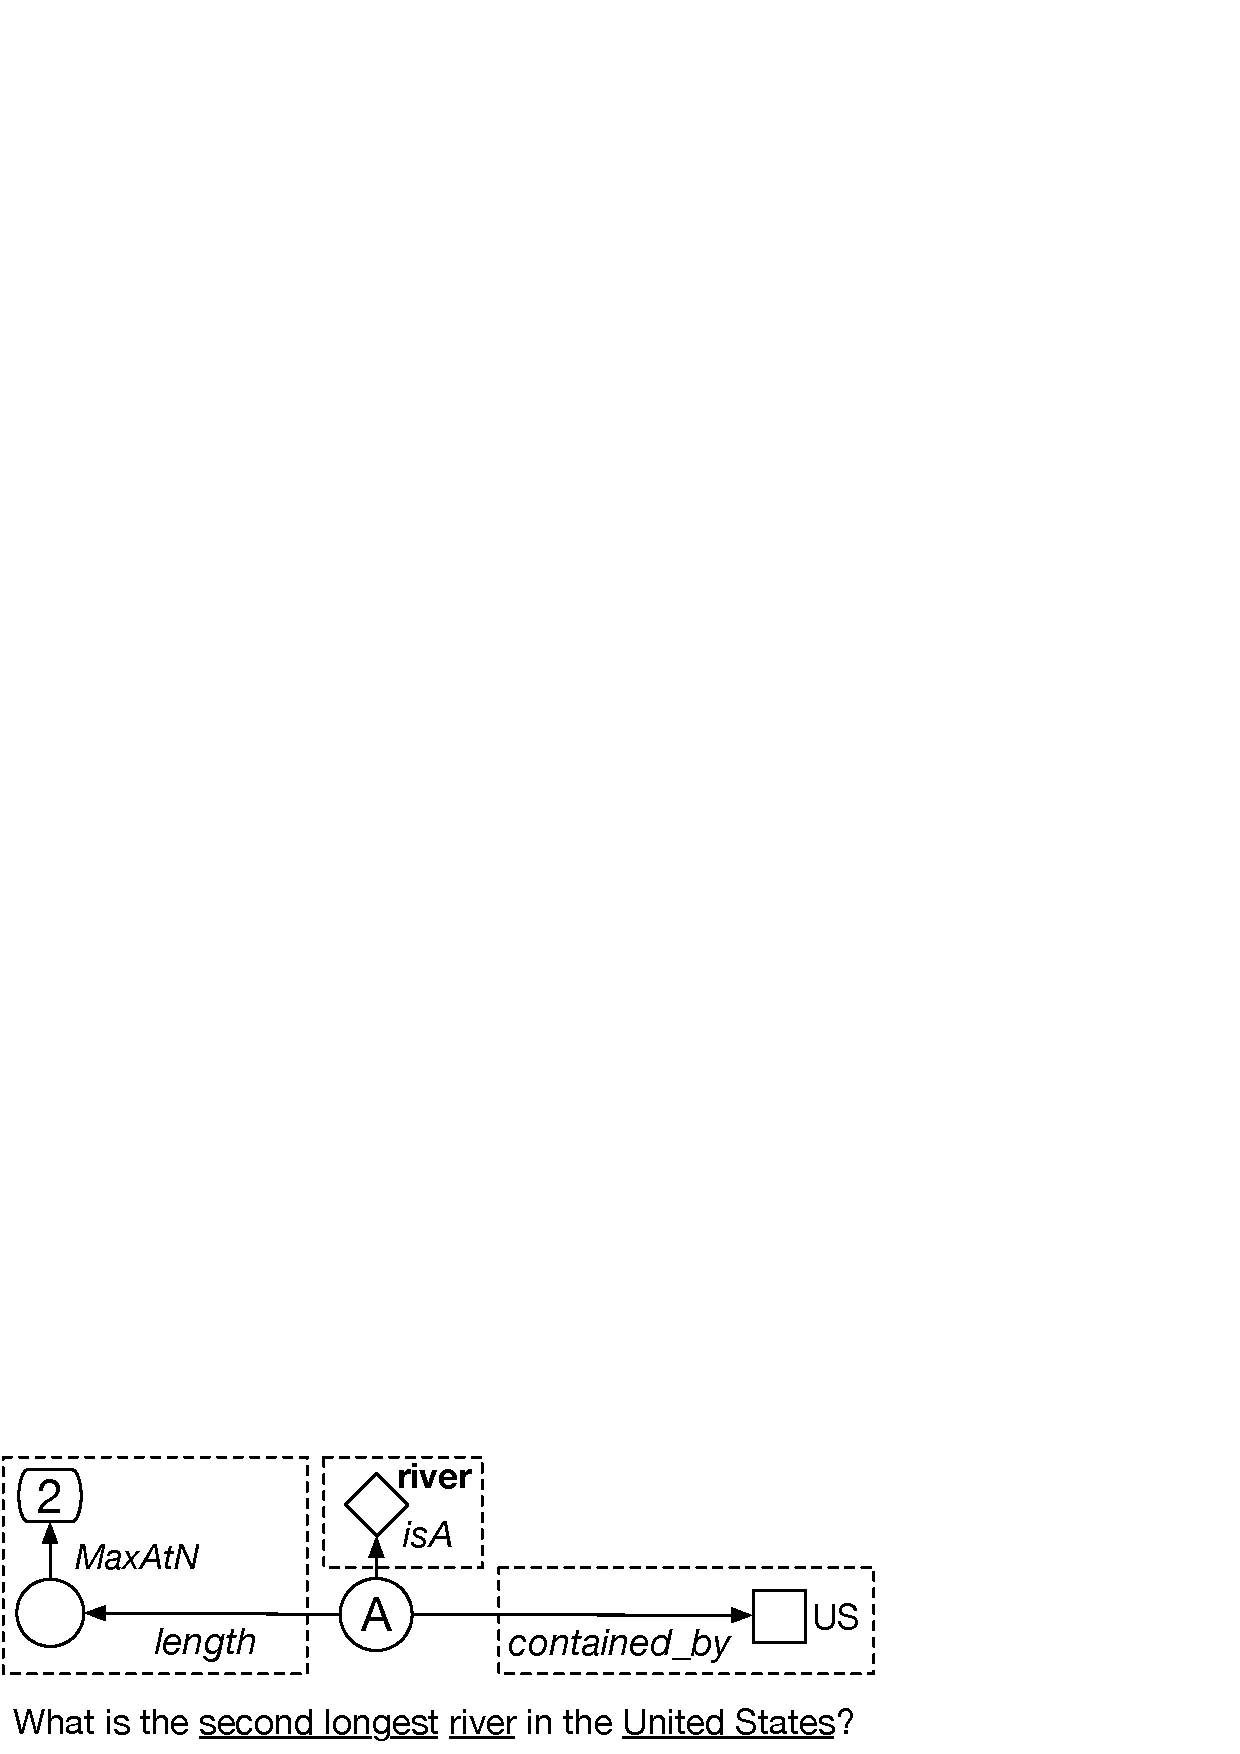
\includegraphics[width=0.43\textwidth]{intro.pdf}
\caption{Item descriptions generation in E-Commerce}
\label{Fig:intro}
\end{figure}


Essentially, EC-IDG problem is to generate sentence-level or paragraph-level descriptions from key words; thus, it can naturally be classified as neural language generation (NLG) problem.
NLG is a theory-motivated range of computational techniques for the automatically generate natural texts in human language.
In the past decades, NLG related tasks have received extensive attention from researchers and significant advance by the rapid development of deep learning.
Recently, NLG has found promise in a variety of applications, such as NMT \cite{bahdanau2014neural}, dialogue systems \cite{lowe2015ubuntu,serban2016building,li2016deep}, abstractive summarization \cite{rush2015neural,paulus2017deep}, poetry generation \cite{zhang2014chinese} and news generation \cite{zhang2016towards}, etc.

\KZ{EC-IDG is a special kind of NLG problem. But I'm sure there are similar
problems of generation text from keywords, that are not specifically for
e-commerce. You need to talk about these and say how is EC-IDG different from
these more generic problems.}
Distinctive from the above-mentioned problems, an input sequence of EC-IDG is a set of dispersed item attributes. % description words.
Source sequences contain but not limited to item name, category, texture, and characteristics, as illustrated in Fig.~\ref{Fig:intro}
\KZ{I suggest removing GMA from the figure because as of now, it's not mentioned
in the intro yet. It was mentioned in abstract but abstract is independent
from the rest of the paper.}
The output description of EC-IDG is expected to be well written sentences 
expanded from input words, denoted as target sequence.
Item description is usually measured from three aspects, including fluency, entity consistency and content attractiveness.
Among them, fluency measures whether the sentences is logically consistent and convey reasonable meaning; 
entity consistency estimate relevance between the description and the entity/key words; 
and lastly, content attractiveness evaluate the attractiveness of the generated content.

The main challenge of EC-IDG is the excessive repetion of words in
the generated text due to the information inequality \KZ{Should you use
the term imbalance of information? The meaning of information inequality is
not clear. This paragraph is very critical in this section so you need to
elaborate the meaning of information inequality and why it leads to 
repetition} between source sequence and target sequence.
The repetiveness becomes especially severe in the scenario of 
long sentence or paragraph generation, and this significantly affects 
sentence quality. \KZ{I don't get the intuition why inequality
in information gives rise to repeition... you need to give some intuition,
probably by examples.}
Target attention \cite{xia2017sequence} and constrained sparsemax \cite{malaviya2018sparse} have been proposed to alleviate this limitation by weighting the hidden states on the target-side generated sentences.
However, these methods can not fully address the problem and the generated descriptions still encounter repetition problem, especially in EC-IDG.

Driven by the above observation, \KZ{What observations? You only observed
that the previous methods didn't work very well. That's not enough for you
to propose a new model. You must have seen something interesting that others
have not seen before..} we propose a novel end-to-end gated memory attention (GMA) network for high-quality E-Commerce item description generation.
As detailed in Figure\ref{Fig:ertgsystem}, the proposed GMA network mainly consists of three modules, including source attention, memory attention and gated selection as well as encoder and decoder module.
There are two memory blocks in memory attention, which preserve previous predictions, i.e., hidden states for final prediction.
During text generation, the proposed GMA first applies source attention to derive the context vector.
Simultaneously, GMA also apply memory attention on the memory blocks independently to acquire their memory vectors. 
After that, GMA merges the context vectors and memory vectors as well as previous prediction knowledge to compute the hidden state and make the final prediction.
Finally, Gated selection module decides which memory block to preserve the hidden state.
\KZ{Intuitively, why does this solution work better?}

The contributions of this paper are summarized as:
\begin{itemize}
\item A new task, namely E-Commerce item description generation (EC-IDG), is introduced to the NLG community. \KZ{Gotta be careful: to say this is the new
task, you must identify the difference between this problem and similar
text generation problems from keywords. Also, if it's a new task, you better
release the dataset for others to try.}
\item A novel gated memory attention (GMA), including source attention, memory attention, and gated selection, is proposed for EC-IDG problem.
\item Memory attention with memory block is proposed to take full advantage of past prediction memory to avoid repetition problem in NLG problem
\item The gated selection module is proposed to decide suitable memory blocks to preserve hidden state of GMA prediction.

\item  The experiments on the EC-IDG demonstrate the superiority of the proposed model over baselines under either manual and artificial metrics. Extended experiments on NMT datasets yield comparable or better performance over previous work, proving the effectiveness and robust of the proposed GMA. \KZ{Better be
 more concrete about how much better you are against the peers.}
\end{itemize}

\section{Related work}
% 参见Towards Constructing Sports News from Live Text Commentary一文
% Generatting text by machine is an existing research field which the industry called it natural language generation(NLG). 
% Our task is similar with news generation, poetry generation. 1 automatically generate sports news from live text commentary scripts. 
% Recurrent neural network is widely used to generate poems that can even confuse readers from telling them from poems written by human poets [7, 8, 11, 33, 37]. NLG also contains conversational systems, abstracts generation and machine translation. Among them, the dialogue system relies on the context information, and the abstract generation needs more input information than the output, both of which have problems of information inequality. In NLG, we want to balance the input and output information to ensure the reliability of the generated text. From this perspective, machine translation is more in line with our task. We can assume that the input information, including keywords, statistical information and other information as the source language, the output as the target language. At the same time NLG in E-commerce has its uniqueness. Item information which NLG need not only the title, but also attributes, a series of information and etc., so the input contains more than news and other fields.
We thought EC-IDG as a kind of NLG related tasks, which include dialog systems, summarization, machine translation,news generation and poetry generation. 

  % Dialog systems relies on the context information to answer the question of human in closed-domain and open-domain. There exists ruler template-based methods \cite{williams2016end,mrkvsic2015multi}, and dialog state tracking\cite{henderson2015machine,wang2013simple} in closed-domain dialog systems. Open-domain system used include IR\cite{isbell2000cobot,ji2014information,yan2016docchat} and Seq2Seq method. Summarization is the task of automatically generating important points from an input document, including centroid based methods, link analysis and graph-based algorithms\cite{erkan2004lexrank,wan2007manifold}, combinatorial optimization techniques such as integer linear programming\cite{gillick2008icsi} and submodular optimization\cite{lin2010multi}. Supervised models have also been adapted which contains learning to rank models\cite{metzler2008machine,shen2011learning,wang2016sentence} and regression\cite{ouyang2007developing,galanis2008aueb}. At the same time neural machine translation (NMT) gained huge success in the last few years\cite{sutskever2014sequence,wu2016google}. \cite{luong2015effective,bahdanau2014neural} introduce attention mechanism to NMT. While many efforts have continued to push the boundaries of recurrent language models\cite{jozefowicz2016exploring}, many other architectures like CNN\cite{gehring2016convolutional,gehring2017convolutional} and self-attention\cite{vaswani2017attention} also bring NMT good results .
  
  % News generation is also a popular area in NLG. In Twitter their study focused on textual summaries for sports events from status updates \cite{nichols2012summarizing}. \cite{tjondronegoro2004highlights} generates sports highlight frames from sports videos. \cite{bouayad2011content}and \cite{bouayad2012perspective}used predefined extraction templates to generate football summaries. \cite{zhang2016towards} automatically generated sports news from live text commentary scripts. Poetry generation is another area in NLG. Traditional approaches for poetry generation include template and grammar-based method\cite{manurung1999chart,oliveira2009automatic,oliveira2012poetryme}. There exists earlier work on generation of poems focusing on style and rhythmic qualities\cite{yan2013poet}. Deep learning approaches is widely used to generate poems that gains better results \cite{ghazvininejad2016generating,ghazvininejad2017hafez,hopkins2017automatically,yi2017generating,zhang2014chinese}. 

  Dialog systems relies on the context information to answer the question of human in closed-domain and open-domain. 
  There exists ruler template-based methods \cite{williams2016end,mrkvsic2015multi}, and dialog state tracking\cite{henderson2015machine,wang2013simple} in closed-domain dialog systems. 
  Open-domain system used IR\cite{ji2014information,yan2016docchat} method. 
  Summarization is the task of automatically generating important points from an input document, including centroid based methods, link analysis and graph-based algorithms\cite{erkan2004lexrank,wan2007manifold}, combinatorial optimization techniques such as integer linear programming\cite{gillick2008icsi} and submodular optimization\cite{lin2010multi}. 
  Supervised models have also been adapted which contains learning to rank models\cite{metzler2008machine,shen2011learning,wang2016sentence} and regression\cite{ouyang2007developing,galanis2008aueb}. 
  At the same time NMT gained huge success in the last few years\cite{sutskever2014sequence,wu2016google}. 
  \cite{luong2015effective} introduce attention mechanism to NMT. While many efforts have continued to push the boundaries of recurrent language models\cite{jozefowicz2016exploring}, many other architectures like CNN\cite{gehring2017convolutional} and self-attention\cite{vaswani2017attention} also bring NMT good results.
  
  News generation is also a popular area in NLG. In Twitter their study focused on textual summaries for sports events from status updates \cite{nichols2012summarizing}. \cite{tjondronegoro2004highlights} generates sports highlight frames from sports videos. \cite{bouayad2012perspective}used predefined extraction templates to generate football summaries. \cite{zhang2016towards} automatically generated sports news from live text commentary scripts. Poetry generation is another area in NLG. Traditional approaches for poetry generation include template and grammar-based method\cite{manurung1999chart,oliveira2012poetryme}. Deep learning approaches is widely used to generate poems that gains better results \cite{ghazvininejad2017hafez,hopkins2017automatically}. 

  Among them, dialogue systems rely on the context information, and summarization systems need more input information than the output. The input and output of NMT always contain the same amount of semantic information. Different from them, a item description contains not only the input information, but also generates some extended information, for example when input is "red T-shirt", the output may be "This is a red T-shirt which makes people who wear it look particularly lively". News generation and poetry generation are more similar to IDG, but news generation is more to describe the number or reality in the language of the news through a certain language structure, and poetry generation is an extension of the semantic level from input, so the requirement for accuracy is not very high.
% 在过去的十年中,通过seq2seq模型进行从序列输入到序列输出的NLP问题代替了统计和语言规则模型。


\section{Models}

% Then we will detail the model we proposed.
Our proposed model follows the RNN based source attention sequence-to-sequence (seq2seq) network that has been widely used for sequence generation. 
In this section, we review the the seq2seq model, including source attention and target attention briefly. The overall framework of \emph{GMA model} will be introduced and represented in Figure~\ref{Fig:ertgsystem}. 

\subsection{Source Attention Seq2seq Model}

RNN based source attention \cite{bahdanau2014neural} seq2seq model mainly contains three components:
 an encoder network,
 a decoder network and an attention model.
 % To better understanding, differentiates 
 Suppose that a source-target sequence pair represents as $(\textbf{x},\textbf{y})$ , where $ \textbf{x}=(x_1,x_2,...,x_I)$ and $ \textbf{y}=(y_1,y_2,...,y_T)$. $I$ and $T$ are the length of source sequence and target sequence respectively. 
 The seq2seq framework reads an input sequence and then translates it to a target sequence word by word. The probability of the translation is modeled as Eq~\eqref{equ:general_loss}. 

\begin{equation}
\label{equ:general_loss}
P(\textbf{y}|\textbf{x})=\prod^T_{t=1 }P(y_t|y_{<t};\textbf{x})
\end{equation}
where $y_{<t}$ represents $\{y_j\}$ in which $j=1,2,3,...,t-1$. 

The encoder network encodes a source sequence into hidden states as shown in Eq~\eqref{equ:encoder_func},
 where $h_i$ is a hidden state mapping to a particular part of the input sequence $\textbf{x}$ and $EncoderRNN(\cdot)$ is an encoder Recurrent Neural Network (RNN). 
 $M^{e}$ represents the source memory buffer at encoder side with size $I$ to store the hidden states and $e(\cdot) \in \mathcal{R}^m $ is an m-dimensional word embedding function.

\begin{equation}
\label{equ:encoder_func}
M^{e}=(h_1,h_2,..,h_I)=EncoderRNN(e(\textbf{x}))
\end{equation}

Source attention is a bridge between encoder network and decoder network and formulated as Eq~\eqref{equ:attn_weight_norm_func} 
where $[I]$ represents the natural number set $\{1,2,...,I\}$. Source attention function $A^e(\cdot)$ calculates the attention factor $\alpha_{t,i}$ with $s_{t-1}$ and $h_i$ as inputs, where $s_{t-1}$ is the previously generated hidden state on target side. In this paper, the attention function is a bilinear function as designed in \cite{paulus2017deep}.
Then a softmax function normalizes the attention factors into attention weights. 

 % normalized attention weight at source side.
\begin{equation}
\label{equ:attn_weight_norm_func}
\alpha_{t,i}=\frac{exp(A^e(s_{t-1},h_{i}))}{\sum_{i=1}^I exp(A^e(s_{t-1},h_{i}))}\ ,\ i \in [I]
\end{equation}

Intuitively, the attention mechanism grants weight $\alpha_{t,i}$ on source-side hidden states $h_i \in M^{e}$ in generating each $c_t^e$ at time step $t$ as follows:
\begin{equation}
\label{equ:contex_vec}
c_t^e=\sum_{i=1}^I \alpha_{t,i}   h_i
\end{equation}

Finally, at the previous time step $t$, the hidden state $s_t$ and the output word are generated by Eq~\eqref{equ:decoder_hidden_func} and Eq~\eqref{equ:decoder_func} respectively. %, where $f(\cdot)$ is a LSTM layer in our model.  

\begin{equation}
\label{equ:decoder_hidden_func}
s_t=RNN(y_{t-1},s_{t-1},c_t^e))
\end{equation}

\begin{equation}
\label{equ:decoder_func}
y_t=g(y_{t-1},s_t,c_t^e)
\end{equation}

The Decoder function $g(\cdot)$ is the combination of a RNN/tanh network and softmax layer. 
At decoding step $t$, the calculation function of generating a target word $y_t$ is Ep~\eqref{equ:decoder_func}. $c_t^e$ is a context vector from encoder side that selectively summarizes certain parts of the source sequence, and $s_t$ is the hidden state on the decoder side.


\begin{figure}[t]
\centering
\includegraphics[width=0.40\textwidth]{attn.pdf}
\caption{Seq2seq network with source attention (green) and target attention (blue).}
\label{Fig:ertgsystem}
\end{figure}

\subsection{Target Attention}

\begin{figure*}[t]
\centering
\includegraphics[width=0.8\textwidth]{v15.pdf}
\caption{Gated memory attention network with source attention, memory attention, gate selection.}
\label{Fig:ertgsystem}
\end{figure*}


Source attention weights the hidden states in source-side memory as mentioned above. 
In contrast, target attention \cite{xia2017sequence} weights the hidden states on target side.
 Similar to the source memory, there is a target-side memory $M^{d}_t={s_1,...,s_{t-1}}$ with size $t-1$ on time step $t$.\
 $M^{d}_t$ contains the components that have been generated so far in the target sequence.
 Target attention weights how important the generated hidden state $s_j$ is, where $j\in [t-1]$.
 The calculation of target attention is shown in Eq~\eqref{equ:targ_attn_weight_norm_func}, where $A^d(\cdot)$ is the attentive function on decoder side. 
% augment the memory space read by decoder RNN by adding an extra target-side memory Mtgt to original source-side one Msrc
\begin{equation}
\label{equ:targ_attn_weight_norm_func}
\beta_{t,j}=\frac{exp(A^d(s_{t-1},s_{j}))}{\sum_{j=1}^{t-1} A^d(s_{t-1},s_{j})}, j\in [t-1]
\end{equation}

Similar to Eq~\eqref{equ:contex_vec}, context vector on decoder side is the weighted sum of hidden states $s_j \in M_{t}^d$: 

\begin{equation}
\label{equ:targ_contex_vec}
c_t^d=\sum_{j=1}^{t-1} \beta_{t,j} s_j, \ j \in[t-1]
\end{equation}

\begin{equation}
\label{equ:targ_contex_vec}
s_t=RNN(s_{t-1},y_{t-1},c_t^e,c_t^d) 
\end{equation}

\begin{equation}
\label{equ:targ_gen}
y_t=g(y_{t-1},s_{t},c_t^e,c_t^d) 
\end{equation}

Afterwards, the new hidden state vector $s_t$ on target side is calculated as shown in Eq~\eqref{equ:targ_contex_vec} with $ c_t^d$ as one of the input elements. 
% 解码生成一个新词的时候,新的隐向量的计算如公式()所示。
Finally, the output word $y_t$ is computed by Eq~\eqref{equ:targ_gen} at time step $t$. 
The target memory $M^{d}$ is updated by pushing the new generated hidden state $s_t$ in: $M^{d}_{t+1} = M_{t}^d \cup {s_t}$. 

\subsection{Gated Memory Attention Model}

In the EC-IDG task, the source sequence is short and the target sequence is much longer. So it is common that several output words attend to the same one input word. Remembering the historical outputs by target side attention is a good strategy to weaken the impact, but it can still be improved.

We find that most repeated words tend to have very similar attention patterns on both source attention and target attention. That is to say, these attention modules lack of a mechanism to avoid repetitive attention patterns. This phenomenon is especially obvious when generate a long sentence.

To end of this, we propose a gated memory attention (GMA) to revise the attention information flow and avoid repetitive attention. 
GMA mainly contains three parts, which are source attention as mentioned before, gated selection for information separation and memory attention for context recall. We will introduce the last two parts later in detail. 

Two attention memories are created to control the previous output information.
Intuitively, we separate the output hidden states into two memory sets. 
In each decoding step $t$, GMA looks at the obtained information ($e(y_{t-1})$, ${s}_{t-1}$, $c^e_t$) and produces a gate value $g_t \in \{0,1\}$ for the coming hidden state $s_{t}$ at the $t^{th}$ step, where 1 means that $s_{t}$ should be pushed to the first memory set (represented by \#$1$) and 0 to the second memory set (represented by \#$0$).

\subsubsection{Memory Attention}

Apart from target-side memory $M^d$, we augment the memory space read by the decoder by adding an extra $M^g$ , which records all the previous generated gate values.
The $t^{th}$ step slice of $M^g$ is $M^g_t=\{g_1,...g_{t-1}\}$.
 After calculating $g_t$, we update the gate memory ${M^g_t}$ by ${M^g_{t}= M^g_{t-1}\cup {g_t}} $ and target-side memory $M^d_t$ by $M^d_{t} \cup {{s}_{t-1}} $.

To decode the $t^{th}$ output, $M^d_t$ is read and masked by the $M^g_t$. We obtain two different target-side memory sets, which are $M^{d_1}_t = M^d_t \circ  M^g_t$ and $M^{d_0}_t = M^d_t \circ (1- M^g_t)$. The two memory sets are weighted averaged separately to generate two contextual representation vectors $c^{d_{1}}_t$ and $c^{d_0}_t$ subsequently, which we call memory vectors.

The memory vectors $c^{d_1}_t$ and $c^{d_0}_t$ on the target side are computed by
\begin{equation}
\label{equ:attentin weight a}
\beta_{t,j}^{d_1} = \frac {exp(A_d(s_{t-1},{s_j}{g_j}))}{\sum_{k=1}^{t-1}{exp(A_d(s_{t-1},{s_k}{g_k}))}}
\end{equation}
\begin{equation}
\label{equ:attentin weight c}
{c^{d_1}_t} = {\sum_{j=1}^{t-1}{\beta_{t,j}^{d_1}}{s_j}{g_j}}
\end{equation}
\begin{equation}
\label{equ:attentin weight b}
\beta_{t,j}^{d_0} = \frac{exp(A_d(s_{t-1},{s_j}{(1-g_j)}))}{\sum_{k=1}^{t-1}{exp(A_d(s_{t-1},{s_k}{(1-g_k)}))}}
\end{equation}
\begin{equation}
\label{equ:attentin weight d}
{c^{d_0}_t} = {\sum_{j=1}^{t-1}{\beta_{t,j}^{d_0}}{s_j}{(1- {g_j})}}
\end{equation}
where $A_d(\cdot)$ is the new attentive function. ${\beta}^{d_1}_{t,j}$ and ${\beta}^{d_0}_{t,j}$ represent the relevancy among output in the $t^{th}$ step and the previous outputs. $c^{d_{1}}_t$ and $c^{d_0}_t$ individually contain information from two different memory sets which the network learns by itself.

Finally, $c^{d_1}_t$ and $c^{d_0}_t$ are fed as two other inputs into the derivation of the final hidden state $s_t$ :
\begin{equation}
\label{equ:final_hidden_func}
s_{t}=LSTM(s_{t-1},y_{t-1},c_t^e,c_t^{d_1},c_t^{d_0}))
\end{equation}

Then we use $s_t$ to compute $y_{t-1}$ through a softmax probability distribution $P(y_t)$ :
\begin{equation}
\label{equ:final_decode}
P{(y_t|y_{<t},\textbf{x})}\propto exp (s_t)
\end{equation}
Several indexes  with the top probabilities in each step are chosen to decide the final output jointly by beam search.

\subsubsection{Gated Selection}

The gate value $g_t$ is computed by Eq~\eqref{equ:gate_func}.
\begin{equation}
\label{equ:gate_func}
g_t = f(e(y_{t-1}),{s}_{t-1},c^e_t)
\end{equation}
where $f(\cdot)$ is a gate function to compute the gate value given all the related inputs.

We have two schemes of the gate function $f(\cdot)$. 
In $f_{Si}(\cdot)$, $g_t$ is achieved by using a single threshold. 
In detail, we firstly compute a score $z_t$ which is similar to the calculation of context gate \cite{Tu:2017:TACL}. 
$z_t$ denotes the confidence of labeling the hidden state $s_{t-1}$ as \#$1$ and is computed by Eq~\eqref{equ:context_gate_func}, where $\sigma$ is a softmax function and $W_z$, $U_z$ and $C_z$ are calculation parameters.
\begin{equation}
\label{equ:context_gate_func}
z_t=\sigma(W_z \cdot e(y_{t-1}),U_z\cdot s_{t-1},C_z \cdot c_t^e))
\end{equation}

Then we use an index function to get $g_t$ in Eq~\eqref{equ:gate index function}, where $\theta$ is defined as a threshold and $mean(\cdot)$ is a function to compute the mean of the vector $z_t$.
\begin{align}
\label{equ:gate index function}
g_t = \begin{cases} 1 & ,\ mean(z_t) \ge \theta \\
					0 &,\ mean(z_t) < \theta
\end{cases}
\end{align}

$f_{Bi}(\cdot)$ computes two confidence scores $z^1_t$ and $z^0_t$ to deciding whether $s_{t-1}$  belongs to the \#$1$ memory set or the \#$0$ memory set. $z^1_t$ and $z^0_t$ are computed by the same equation as Eq~\eqref{equ:context_gate_func} but are with individual layer parameters. The two scores, i.e. $z^1_t$ and $z^0_t$, compete with each other when making a decision. When $z^1_t \geq z^0_t$, we judge the hidden state $s_{t-1}$ to belong to \#$1$ set, and vice versa. This process is defined as shown in Eq~\eqref{equ:bi gate index function}.
\begin{align}
\label{equ:bi gate index function}
g_t = \begin{cases} 1 & ,\ mean(z_t^1) \ge mean(z_t^0) \\
					0 &,\ mean(z_t^1) < mean(z_t^0)
\end{cases}
\end{align}

The gate selection creates two attention contexts, making the previous output information split-flow and thus reduce the impact of the length of long sentence in the decoding process.

% Intuitively, in each decoding step $t$, GMA looks at the obtained information ($e(y_{t-1})$, ${s}_{t-1}$, $c^e_t$) and produces a gate value $g_t \in \{0,1\}$ for the coming output word $y_{t}$ at the current step, where 1 denotes that the $y_{t}$ belongs to the entity word set and 0 denotes that $y_{t}$ belongs to the derivative word set. The gate number $g_t$ is computed by Eq~\eqref{equ:gate_func}.
\section{Evaluation Metrics}
\subsection{Automatic Evaluation}

To evaluate the proposed method, we report the tokenized 4-gram BLEU \cite{papineni2002bleu} and ROUGE-L (referred as ROUGE later) \cite{lin2004rouge}, repetition score (Rep) \cite{malaviya2018sparse} as well as a new metric that describes below.

\subsubsection{Repetition Score}

Repetition score is used to count the repeated words of the generated sentences. Formally, given an n-gram $w^n \in { V }^{ n }$ and a frequency function $q(\cdot)$. Let $q(w^n,\textbf{y})$ and $q(w^n,\textbf{r})$ be the the frequency of $w^n$ in the model translation and reference. The sentence level score $\sigma (\textbf{y},\textbf{r})$ is firstly computed as
\begin{align}
\label{equ:sentence-level score}
\sigma (\textbf{y},\textbf{r})=\sum^n_{k=1}{\sum_{w^k\in V^k }{\lambda_k  max\{ 0, \delta(w^k,\textbf{y},\textbf{r} )\}}}
\end{align}
where is $\delta(w^k,\textbf{y},\textbf{r}) = q(w^k,\textbf{y})-q(w^k,\textbf{r})$.
Repetition score is then given by summing $\sigma(\textbf{y}, \textbf{r})$ over sentences, normalizing by the number of words on the reference corpus, and multiplying by 100. We follow the setting of $n=2, \lambda_{1}=1$ and $\lambda_{2}=2$ in \cite{malaviya2018sparse}.
\subsubsection{Coverage Rate}
In EC-IDG, we always expect to make full use of all the input information. 
We use a metric named coverage rate to evaluate how many words in the source sequence are covered by the generated sequence.
Given 1-gram word set $ {s(\textbf{x})}$ and ${s(\textbf{y})}$ of source sequence and target sequence,
 the sentence level coverage rate $\gamma(\textbf{y}, \textbf{x})$ is given by
\begin{equation}
\label{coverage rate}
\gamma(\textbf{y}, \textbf{x}) = \frac {s(\textbf{x})\bigcap s(\textbf{})}{s(\textbf{x})}
\end{equation}

Same as repetition score, we compute the average sentence level coverage rate among all sentences in the test set.

\subsection{Side-by-side human annotation}
We also conduct human evaluations to judge readability of the generated descriptions. 
To each annotator, we showed the source attributes and the item descriptions generated by different methods. 
The human evaluator does not know each description comes from which model. 
Three scores from 0-5 are assigned to each description, one for fluency, one for consistency and the last one for attractiveness. Each description is rated by 12 different human evaluators and the results are averaged across all the descriptions and evaluators. The following is the criteria:
\begin{itemize}
\item Fluency: A fluent description should be language coherence, logically consistent, meaning reasonable and without repetition;
\item Consistency: The description should logically be consistent to the attribute/key words in the source sequence. If a description is either irrelevant or logically contradictory to the input context, it can be judged to be inconsistent;
\item Attractiveness : This metric is to measure the purchasing desire when seeing the commodity item description.
\end{itemize}

\section{Experiments and Datasets}
%\subsection{ Training details }
% We train 2-layer LSTMs of 512 units with 1 bidirectional layers for the encoder, embedding dim is 512. Attention is used with dropout rate of 0.2. All parameters are uniformly. We use SGD with learning rate 1.0 as follows: train for 10K steps (about 10 epochs); after 8K steps, we start halving learning rate every 1K step.
\subsection{Experimental Setup}
We trained a bidirectional encoder network with 2-layer LSTMs of 512 hidden units. The embedding dimension is 512. The dropout rate is set to be 0.2 in the LSTM layer. All parameters are uniformly initialized. We use SGD optimizer with initial learning rate 1.0 to train the models.
 
Experiments were carried out on the two variants of our GMA about the gate function. GMA-Si and GMA-Bi denotes the proposed method with $f_{Si}(\cdot)$ and $f_{Bi}(\cdot)$ as the gate function respectively. We also compare with the base (original source attention seq2seq model) and the Tgt-Att (base + target side attention) to prove the effectiveness of our method.

\subsection{Experiments on EC-IDG datasets.}

\begin{table}[h]
\renewcommand\arraystretch{1.1}
\small
\vspace{1mm}
\begin{tabular}{c|c|c|c|c|c}
\hline
          & inp-len & opt-len & \#train & \#valid  & \#test \\ \hline
clothes   & 6-10         & 31-50         & 214,176   & 5000      & 5000     \\ \hline 
shoes     & 4-7          & 21-30         & 254,464   & 5000      & 5000     \\ \hline
furniture & 6-10         & 21-50         & 233,133   & 5000      & 5000    \\ \hline
\end{tabular}
\caption{Detailed information for the EC-IDG datasets.}
\label{table:IDG dataset}
\end{table}

% \begin{table*}[]
% \centering{}
% \renewcommand\arraystretch{1.2}
% \small
% \vspace{1mm}
% \begin{tabular}{|l|l|}
% \hline
% \begin{CJK}{UTF8}{gkai}
% 甜美 斗篷 花朵 刺绣 文艺 
% \end{CJK} 
% &  
% \begin{CJK}{UTF8}{gkai}
% 很文艺甜美的一款斗篷外套,精致的花朵刺绣点缀衣 身,文艺又能轻易俘获人心 。     
% \end{CJK}
% \\ \hline
% \begin{tabular}[c]{@{}l@{}}
% Sweet, cloak, flowers, embroidery, \\ art
% \end{tabular}  
% & 
% \begin{tabular}[c]{@{}l@{}}
% It is a very literary and sweet cloak jacket; Delicate flower embroidery embellishes the body, \\ which makes the clothes in art fashion and charming.
% \end{tabular}  
% \\ \hline
% \begin{tabular}[c]{@{}l@{}}
% \begin{CJK}{UTF8}{gkai}
% 乳白色 毛衣 羊驼毛 纯净 舒适 
% \end{CJK}
% \end{tabular} 
% & 
% \begin{tabular}[c]{@{}l@{}}
% \begin{CJK}{UTF8}{gkai}
% 温柔的乳白色毛衣,细腻的羊驼毛配上纯净的颜色,上身保暖舒适,而且还能轻松\end{CJK} \\ \begin{CJK}{UTF8}{gkai} 穿出女神范。\end{CJK}
% \end{tabular} 
% \\ \hline
% \begin{tabular}[c]{@{}l@{}}Milky white, sweater, alpaca hair, \\ pure, comfort
% \end{tabular} 
% & 
% \begin{tabular}[c]{@{}l@{}}
% A sweet milky white sweater with delicate alpaca hair in pure color , is warm and comfortable, \\ which makes people in full-on goddess style easily.
% \end{tabular} 
% \\ \hline
% \end{tabular}
% \caption{Examples of Chinese Generated Item Description with Input (left) and Output (right)}
% \label{tabel: example}
% \end{table*}
\begin{table*}[]
\centering{}
\renewcommand\arraystretch{1.2}
\small
\vspace{1mm}

\begin{tabular}{|p{0.52\textwidth}|p{0.42\textwidth}|}
\hline
Tgt-Attn
 & GMA-Si
\\ \hline
\begin{CJK}{UTF8}{gkai}经典时尚的裁剪,复古怀旧怀旧怀旧怀旧怀旧怀旧怀旧怀旧怀旧怀旧怀旧怀旧怀旧怀旧怀旧怀旧怀旧怀旧怀旧怀旧怀旧怀旧怀旧怀旧怀旧怀旧怀旧怀旧蓝,裤子有弹性,上身很舒服。
\end{CJK} 
 & \begin{CJK}{UTF8}{gkai}时尚九分裤型裁剪,复古怀旧中蓝,裤子的弹性很好,穿起来很舒服。 \end{CJK}                                                            
  \\ \hline
\begin{CJK}{UTF8}{gkai}高腰剪裁,拉长身高比例,穿出高挑感。拉链设计,方便穿脱,隐形拉链设计,方便穿脱,穿脱方便。   \end{CJK}                                                         & 
\begin{CJK}{UTF8}{gkai}高腰剪裁,拉长身高比例,更显高挑,腰头拉链设计,方便穿脱,腰侧隐形侧拉链,穿着更加便利。 \end{CJK}                                                
\\ \hline
\begin{CJK}{UTF8}{gkai}袖口和下摆的收紧设计,增加了衣服的时尚感,同时也增加了衣服的时尚感,宽松的廓形设计,整体的走线,提升了衣身的指数。 \end{CJK}
& 
\begin{CJK}{UTF8}{gkai}袖口和下摆的撞色螺纹设计,提升层次感的同时更显宽松。整体的剪裁和走线都非常精致,吸睛指数max。\end{CJK} 
\\ \hline
\end{tabular}
\caption{Examples of Chinese Generated Item Description with Tgt-Attn(left) and GMA-Si (right)}
\label{tabel: example}
\end{table*}

\begin{table*}[]
%\normalsize
\centering{}
\renewcommand\arraystretch{1.1}
\small
\vspace{1mm}
\begin{tabular}{c|c|c|c|c|c|c|c|c|c|c|c|c}
\hline
         & \multicolumn{4}{c|}{Clothes}                                     & \multicolumn{4}{c|}{Shoes}                                        
         & \multicolumn{4}{c}{Furniture}                                   \\ \cline{2-13}
         & BLEU            & ROUGE          & Rep            & Cover           & BLEU            & ROUGE           & Rep             & Cover               & BLEU            & ROUGE          & Rep             & Cover           \\ \hline
base     & 49.75           & 68.92           & 3.39           & 94.88           & 56.94           & 74.18           & 0.94            & 96.74            
         & 42.64           & 68.13           & 2.30           & 94.68           \\ \hline
Tgt Attn & 49.08           & 68.39           & 2.75           & 94.09           & 56.92           & 74.31           & 0.98            & 96.77              & 42.21          & 68.12          & 2.19          & 94.70          \\ \hline
GMA-Si   & 49.97           & 69.05          & \textbf{2.72}   & 94.80           & 56.97           & 74.43           & \textbf{0.84} & \textbf{96.79}        & \textbf{43.43}   & \textbf{68.57}  & \textbf{2.03}  & \textbf{94.76} \\ \hline
GAM-Bi   & \textbf{50.04}  & \textbf{69.19} & 2.74            & \textbf{94.90}  & \textbf{57.21}  & \textbf{74.53}  & 0.86           & \textbf{96.79}      & 43.15          & 68.45          & 2.08          & 94.63          \\ \hline
\end{tabular}
\caption{Experimental results on EC-IDG dataset.}
\label{tabel: IDGexp}
\end{table*}


\begin{table}[]
\centering
\renewcommand\arraystretch{1.1}
\small
\begin{tabular}{c|c|c|c}
\hline
         & Fluency       & Consistency   & Attractiveness    \\ \hline 
base     & 3.67          & 4.00          & 3.61          \\ \hline
Tgt-Attn & 3.78          & 4.07          & 3.68          \\ \hline
GMA-Si   & 3.82          & 4.03          & 3.79          \\ \hline
GMA-Bi   & \textbf{3.91} & \textbf{4.08} & \textbf{3.87} \\ \hline
\end{tabular}
\caption{Human evaluation score on a random subset of the EC-IDG-clothes dataset.}
\label{table: manually evalue}
\end{table}

\subsubsection{EC-IDG Datasets}

We collected item description sequence pairs from three E-Commerce scenarios, including clothes, shoes and furniture.
Item attributes were set as the source input sequence, and Item descriptions were originally produced by experienced people. 
Sequence pairs that are too long or too short were filtered out according to the distribution of raw collected data.
The detailed information of the three filtered datasets are listed in Table \ref{table:IDG dataset}.

\subsubsection{Experimental Results}
Table \ref{tabel: IDGexp} shows the EC-IDG performance in terms of BLEU, ROUGE, repetition score (Rep), and coverage rate (Cover).

We can observe that GMA-Si and GMS-Bi have their individual advantage in different datasets. GMA-Si always has the best repetition scores. 
And the GMA-Bi takes the second position about repetition. These facts prove the effectiveness in reducing the repeated word by separately using the previous hidden state histories in our GMA. On BLEU, ROUGE and coverage rate, GMA-Bi performs the best in the clothes and shoes datasets. And GMA-Si wins the first place in the furniture datasets. But in total, the metric results of GMA-Si and GMS-Bi are very close.

The length of sentences in the furniture dataset is more diverse than that in the clothes and shoe datasets. 
To this end, GMA performs better in a multivariate condition but GMA learns better expression ability in the dedicated task. 
Experimental results show that GMA with a stationary threshold (GMA-Si) is more stable and with two constantly changing scores (GMA-Bi) is more adaptive. Overall, GMA-Si and GMA-Bi obviously outperform the base and Tgt-Attn methods, which proves the validation of our gated memory attention mechanism.

On the three EC-IDG datasets, we find that Tgt-Attn outperforms the base method on the repetition rate by a large margin. 
This is because Tgt-Attn considers the previous output information when generating item descriptions. 
But the BLEU of Tgt-Attn is a little bit lower than base. 
The ROUGE score is comparable with base on the shoe and furniture datasets but is also a little worse than base. 
We think that the
integrating information method on target side
as Tgt-Attn
makes the network 
focus on 
not only the relevant information but also the redundancy, 
causing slightly worse expression ability.

\KZ{You show the good cases in table 2. Are there any bad cases? Are
repetition completely eliminated? If not, for those base cases, can you
give a bit of error analysis to explain why you method works most of the times
and doesn't work the rest of the times? I also think instead of showing results
of GMA-Si and GMA-Bi, which are two variants, also give some kind of ablation
tests that help readers understand what are the most critical components in
your model that make things better.}
Comparison results of human evaluation on a random subset of the clothes dataset are summarized in Table \ref{table: manually evalue}.
It is obvious to see that the descriptions generated by GMA-Bi achieve highest scores in terms of the three aspects. 
GMA-Si is also superior than both Tgt-Attn and base methods on fluency and attractiveness. 
% Our overwhelming 
Human evaluation results show that GMA net has overwhelming advantage over baselines,
which certifies that our method does improve readability.

\KZ{I notice that there's no quantitative results on repeatness. I think this
should be done somehow since this is your major target! Should include another
column in Table 4.}

\begin{table*}[h]
\centering
% \centering
\renewcommand\arraystretch{1.1}
\small
\vspace{1mm}
\begin{tabular}{c|c|c|c|c|c|c|c|c}
\hline
  & \multicolumn{2}{c|}{En-Fr} & \multicolumn{2}{c|}{Fr-En} & \multicolumn{2}{c|}{En-Vi} & \multicolumn{2}{c}{Vi-En} \\ \cline{2-9} 
\multirow{-2}{*}{} & BLEU  & Rep & BLEU  & Rep  & BLEU  & Rep  & BLEU  & Rep  \\ \hline
% \rowcolor[HTML]{ECF4FF} 
Base \cite{bahdanau2014neural} & 32.09 & 2.49 & 29.54 & 2.40  & 24.81 & \textbf{3.01 } & 18.69 & 6.39  \\ \hline
% Context Gate  & 25.68 & 6.21 & 25.92 & 6.52  & 24.11 & 7.18  & 19.47 & 8.62  \\ \hline
% \rowcolor[HTML]{ECF4FF} 
Tgt-Attn  & 33.05 & 2.53 & 29.54 &\textbf{ 2.03 } & 23.30 & 3.21  & 20.20 & 3.46  \\ \hline
% Bi-Trg Attn & 32.23 & 4.02 & 27.34 & 7.48  & 23.34 & 6.02  & 16.63 & 14.89 \\ \hline
% \rowcolor[HTML]{ECF4FF} 
GMA-Si & 34.10 & 2.50 & 30.90& 2.26&\textbf{24.88}&3.79 & \textbf{20.98} & 4.32  \\ \hline
% \rowcolor[HTML]{ECF4FF} 
GMA-Bi  & \textbf{35.24} & \textbf{2.29} &\textbf{30.94} & 2.48 &24.49 &3.98 & 20.52 & \textbf{4.27}\\ \hline
\end{tabular}
\caption{Experimental Results on NMT datasets}
\label{table:NMTexp}
\end{table*}

Several generated item description examples are listed in Table~\ref{tabel: example}.
GMA-Si can produce fluent, coherent and smooth descriptions, which are close to human written level.

\subsection{Experiments Details on NMT}

To see the effectiveness and robustness of our method, we also conduct extended experiments on the NMT datasets.
\subsubsection{NMT Datasets}
We evaluated our proposed method on four language pairs from IWSLT  English-French (En-Fr), French-English (Fr-En), English-Vietnamese (En-Vi) and Vietnamese-English (Vi-En) corpus.
%The International Workshop on Spoken Language Translation is a yearly event associated with an open evaluation campaign on spoken language translation. IWSLT proposes every year challenging research tasks and an open experimental infrastructure for the scientific community working on spoken and written language translation.

The training sets have 280,646 and 143,353 parallel sentences for IWSLT 2017 En-Fr / Fr-En and IWSLT 2015 En-Vi / Vi-En data, respectively.
For En-Fr / Fr-En experiments, we use 2014 test sets (1,188 sentences) as the development sets and 2015 test sets (1,210 sentences) as test sets. For En-Vi / Vi-En experiments, the developing sets and testing sets are 2012 test sets (971 sentences) and 2013 test sets (1,268 sentences) respectively.

We use $tokenize.perl$ script and followed \cite{cettoloEtAl:EAMT2012} to split words into subword units. In training, sentences have more than 50 words were discarded.
%The paper reports the case-sensitive tokenized BLEU score for all datasets.
\subsubsection{Experimental Results}
The experimental results on NMT datasets are presented in the Table \ref{table:NMTexp}. 
We can see that GMA-Bi achieves best BLEU scores in the En-Fr / Fr-En translation experiments, and GMA-Si performs best in En-Vi / Vi-En translation task. 
This proves that GMA is beneficial to the expression learning ability of the network. 
Our methods has the best repetition score in En-Fr experiments. 
But the repetition scores of our methods are inferior than the comparison methods on other tests. 
The reason is that translation task if different from EC-IDG task. 
In translation task, input and output mostly have a one-to-one corresponding relationship, making the task more associate with source attention and that has the problem of the long output sentence. 
Therefore, the Tgt-Attn with one target memory works well.

\section{Conclusion}


In this paper we introduced a new task for EC-IDG.
The study focused on the task and proposed an end to end model, which named GMA. 
There are three components in GMA, i.e., source attention, memory attention and gated selection. 
The GMA mechanism can reduce the repetition in target sequence by considering the similarity of attention patterns gated selection in long generated sequence, and thus the fluency is promoted. 
Experimental results on EC-IDG datasets demonstrate that the proposed method can promote the quality of generation sentences by both side-by-side human annotation and machine evaluation. 
Extended experiments on NMT datasets yield comparable or better performance over previous work, which proves the effectiveness and robustness of the proposed GMA.

Avenues for future work are many and varied.
Additional research should focus not only upon the repetition of target sentences. We would like to generate more attractive and accurate descriptions of items. And we hope that some of the proposed work might be of relevance to other generation tasks such as poem generation, news generation and dialogue systems.
% Especially, Such research can estabilish 
\bibliographystyle{aaai}
\bibliography{refs}
\end{document}
